% Template file to use for LLNCS papers prepared in LaTeX
\documentclass{llncs}
\usepackage{hyperref}
\usepackage{amsmath}
\usepackage{graphicx}
\usepackage{listings}
\usepackage{paralist}
\usepackage{xcolor}
\usepackage[]{algorithm2e}
\colorlet{punct}{red!60!black}
\definecolor{background}{HTML}{EEEEEE}
\definecolor{delim}{RGB}{20,105,176}
\colorlet{numb}{magenta!60!black}


% JSON listings
\newcommand{\linenumberstyle}{\scriptsize}
\lstdefinelanguage{json} {
  sensitive=false,
  morestring=[b]"',
  showstringspaces=false
}
\lstset{
  numberbychapter=false,
  language=json,
  basicstyle=\scriptsize\ttfamily,
  captionpos=b,
  % keywordstyle=\color[rgb]{0,0,0.7},
  % stringstyle = \color[rgb]{0,0.5,0},
  % identifierstyle=\color{orange},
  commentstyle=\color[gray]{0.5},
  backgroundcolor=\color[gray]{0.96},
  framexleftmargin=1pt,
  xleftmargin=4.4pt,
  xrightmargin=3.4pt,
  numbers=left,
  breaklines=true,
  numberstyle=\linenumberstyle,
  frame=single,
  aboveskip=1.3em,
  inputencoding=utf8,
  extendedchars=true,
   literate=
     *{0}{{{\color{numb}0}}}{1}
      {1}{{{\color{numb}1}}}{1}
      {2}{{{\color{numb}2}}}{1}
      {3}{{{\color{numb}3}}}{1}
      {4}{{{\color{numb}4}}}{1}
      {5}{{{\color{numb}5}}}{1}
      {6}{{{\color{numb}6}}}{1}
      {7}{{{\color{numb}7}}}{1}
      {8}{{{\color{numb}8}}}{1}
      {9}{{{\color{numb}9}}}{1}
      {:}{{{\color{punct}{:}}}}{1}
      {,}{{{\color{punct}{,}}}}{1}
      {\{}{{{\color{delim}{\{}}}}{1}
      {\}}{{{\color{delim}{\}}}}}{1}
      {[}{{{\color{delim}{[}}}}{1}
      {]}{{{\color{delim}{]}}}}{1},
}

\renewcommand{\lstlistingname}{Code}

\newcommand{\furl}[1]{\footnote{\scriptsize \url{#1}}} 
\def\sectionautorefname{Section}

\begin{document}
\title{Linked Data Reactor: a Framework for Building Reactive Linked Data Applications}
\titlerunning{Linked Data Reactor}

\author{Ali Khalili}
\authorrunning{Ali Khalili}

\institute{%
Knowledge Representation and Reasoning Research Group\\Deptartment of Computer Sciences\\ Vrije Universiteit Amsterdam\\
\email{a.khalili@vu.nl}
}
\maketitle

\begin{abstract}
This paper presents Linked Data Reactor (LD-Reactor or LD-R) as a framework for developing flexible and reusable User Interface components for Linked Data applications. LD-Reactor utilizes Facebook's ReactJS components, Flux architecture and Yahoo's Fluxible framework for isomorphic Web applications. It also exploits Semantic-UI framework for flexible UI themes. LD-R aims to apply the idea of component-based application development into RDF data model hence enhancing current user interfaces to view, browse and edit Linked Data. \newline

Documentation: \url{http://ld-r.org} \newline
Demo: \url{http://demo.ld-r.org} \newline
Code Repository: \url{https://github.com/ali1k/ld-r}

\end{abstract}

\section{Introduction}


With the growing number of structured data published, the Web is moving towards becoming a rich ecosystem of machine-understandable Linked Data.
Semantically structured data facilitates a number of important aspects of
information management such as information retrieval, search, visualization, customization, personalization and integration~\cite{SCAJ-Khalili-2013}.
Despite all these benefits, Linked Data Applications (LDAs) are not yet adopted by the large community of Web developers outside the Semantic Web domain and, causally, by the end-users on the Web.

The current communication gap between Semantic Web developers and User Experience (UX) designers, caused by the need to bear Semantic Web knowledge, prevents the streamlined flow of best practices from the UX community into Linked Data user interface (UI) development.
The resulting lack of adoption and standardization often makes current LDAs inconsistent with user expectations and impels more development time and costs on LDA developers.
In this situation, more time is spent in re-designing existing UIs rather than focusing on innovation and creation of sophisticated LDAs.

In \cite{khaliliLDR2016}, We performed an elaborate study on the current pitfalls of LDA UI design and proposed \emph{Adaptive Linked Data-driven Web Components} and its open source implementation called Linked Data Reactor\footnote{\url{http://ld-r.org}} as a solution to tackle those issues. This paper serves as a more technical description of that idea.

\section{Adaptive Linked Data-driven Web Components}
In order to streamline the process of UI development in LDAs, we propose an architecture of adaptive LD-R Web components -- Web components enriched by the RDF data model.
As shown in \autoref{fig:framework}, the proposed architecture addresses LDA UI reusability and flexibility by incorporating RDF-based Web components and scopes.
In the following sections, the main elements of the architecture are described:

\subsection{LD-R Web Components}
As depicted in \autoref{fig:architecture}, there are four core component levels in an LD-R Web application.
Each core component abstracts the actions required for retrieving and updating the graph-based data and provides a basis for user-defined components to interact with Linked Data in three modes: view, edit and browse.
%For example, a viewer in the level of \emph{Dataset} component can enable visualizing a set of resources based on a certain property value whereas a viewer in the level of \emph{Resource} component can only allow visualizing properties of a specific resource (or a specific type of resource).

\begin{figure}[htb]
	\center
  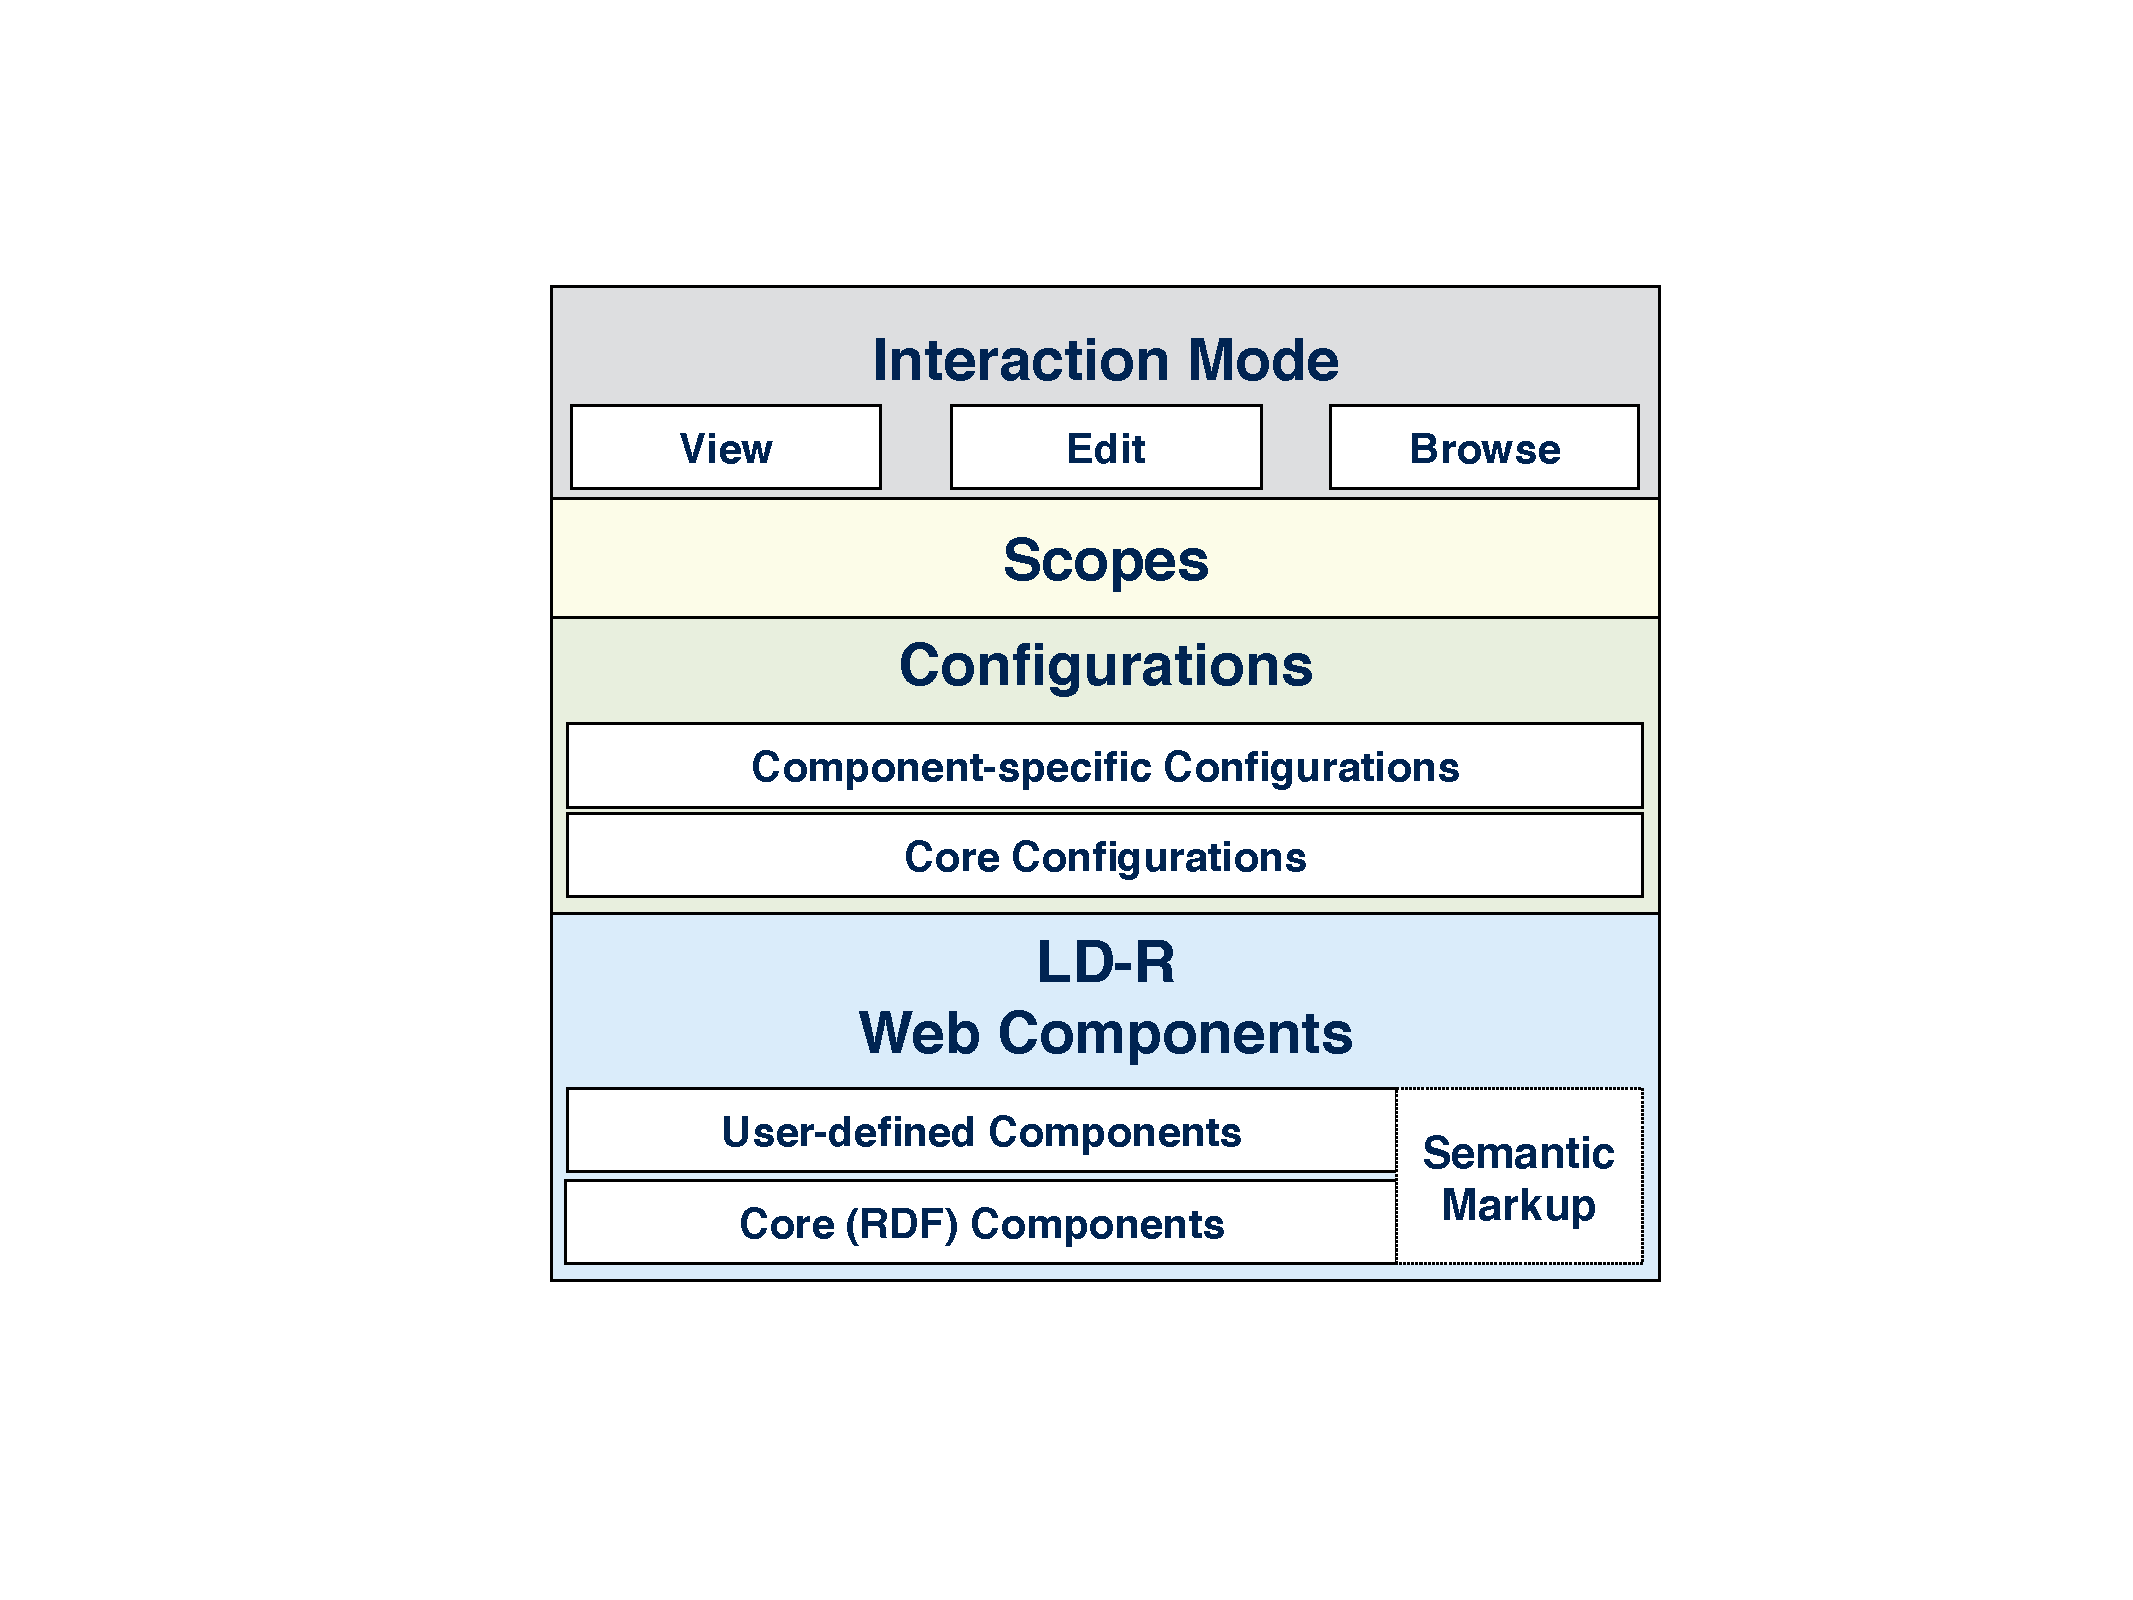
\includegraphics[width=0.80\linewidth]{images/framework.pdf}
  \caption{Main elements of the adaptive LD-R Web components architecture.}
  \label{fig:framework}
\end{figure}

\begin{figure}[htb]
  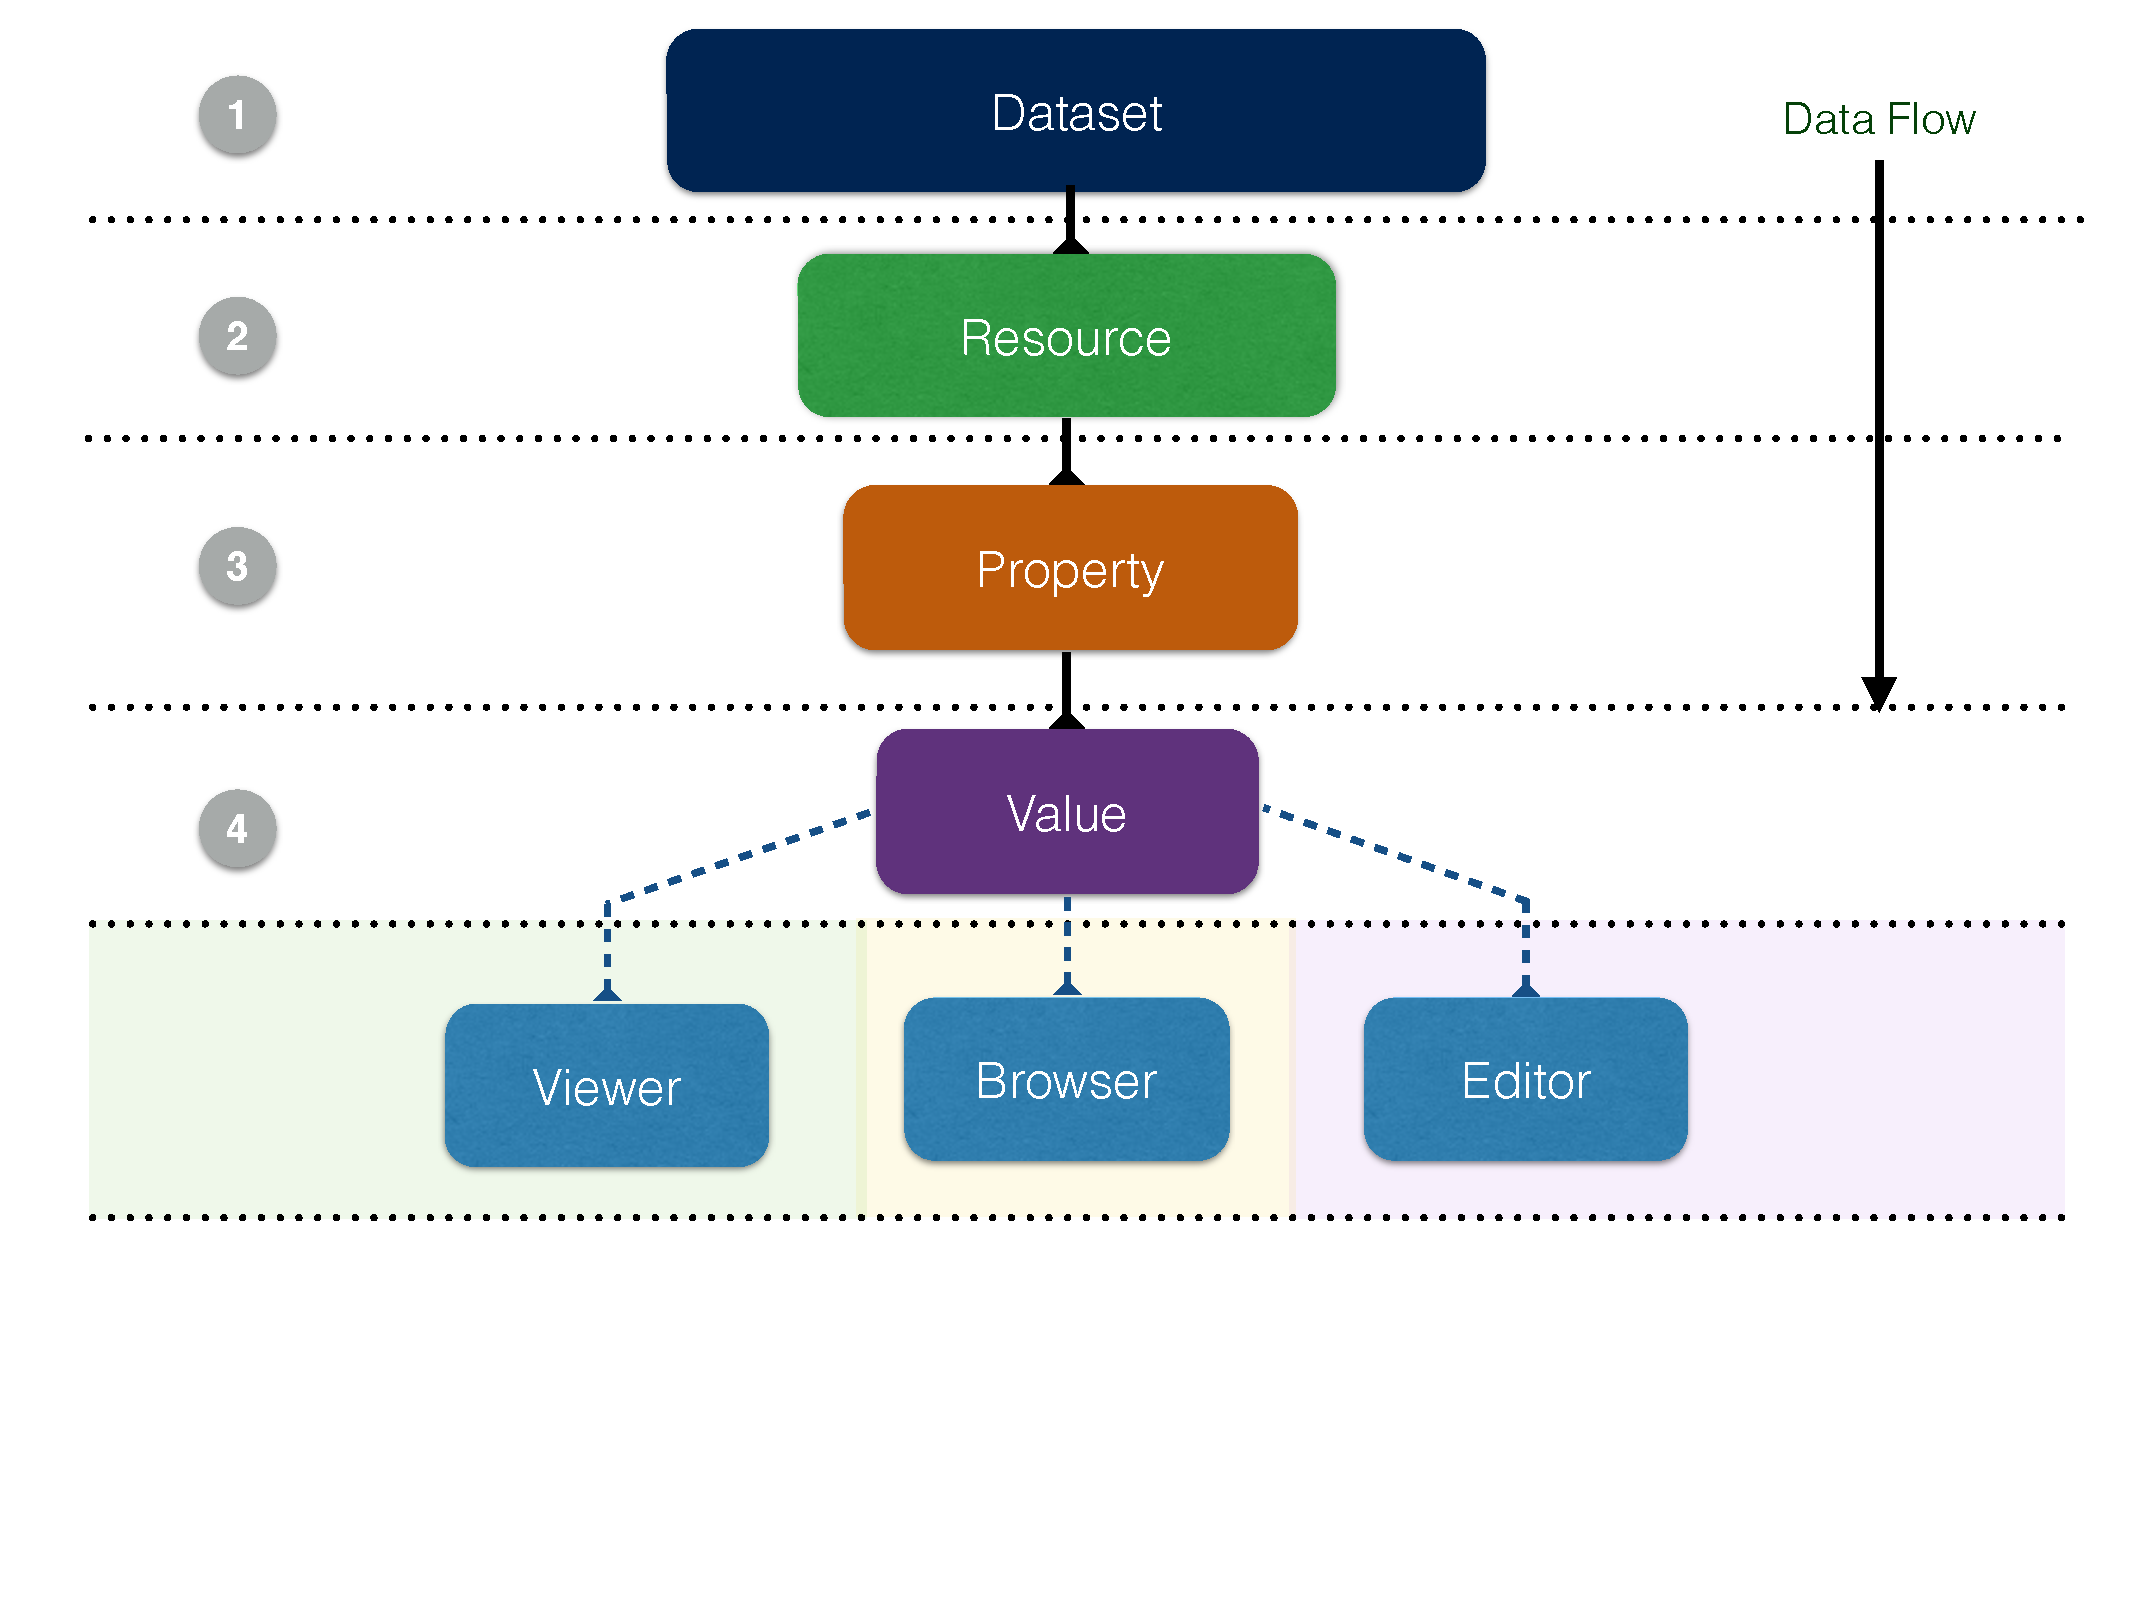
\includegraphics[width=1\linewidth]{images/architecture.pdf}
  \caption{Core LD-R Web components.}
  \label{fig:architecture}
\end{figure}

The data-flow in the system starts from the \emph{Dataset} component which handles all the events related to a set of resources under a named graph identified by a URI.
The next level is the \emph{Resource} component which is identified by a URI and indicates what is described in the application.
A resource is described by a set of properties which are handled by the \emph{Property} component.
Properties can be either individual or aggregate when combining multiple features of a resource (e.g. a component that combines longitude and latitude properties; start date and end date properties for a date range, etc.).
Each property is instantiated by an individual value or multiple values in case of an aggregate object.
The value(s) of properties are controlled by the \emph{Value} component.
In turn, Value components invoke different components to view, edit and browse the property values.
\emph{Viewer}, \emph{Editor} and \emph{Browser} components are terminals in the LD-R single directional data flow where customized user-generated components can be plugged into the system.
%These components apply on individual and aggregate values in different levels.
 %(e.g. to show multiple coordinates on a map).
User interactions with the LD-R components are controlled by a set of configurations defined on one or more selected component levels known as scopes.

\subsection{Scopes and Configurations}

\begin{figure}[tb]
  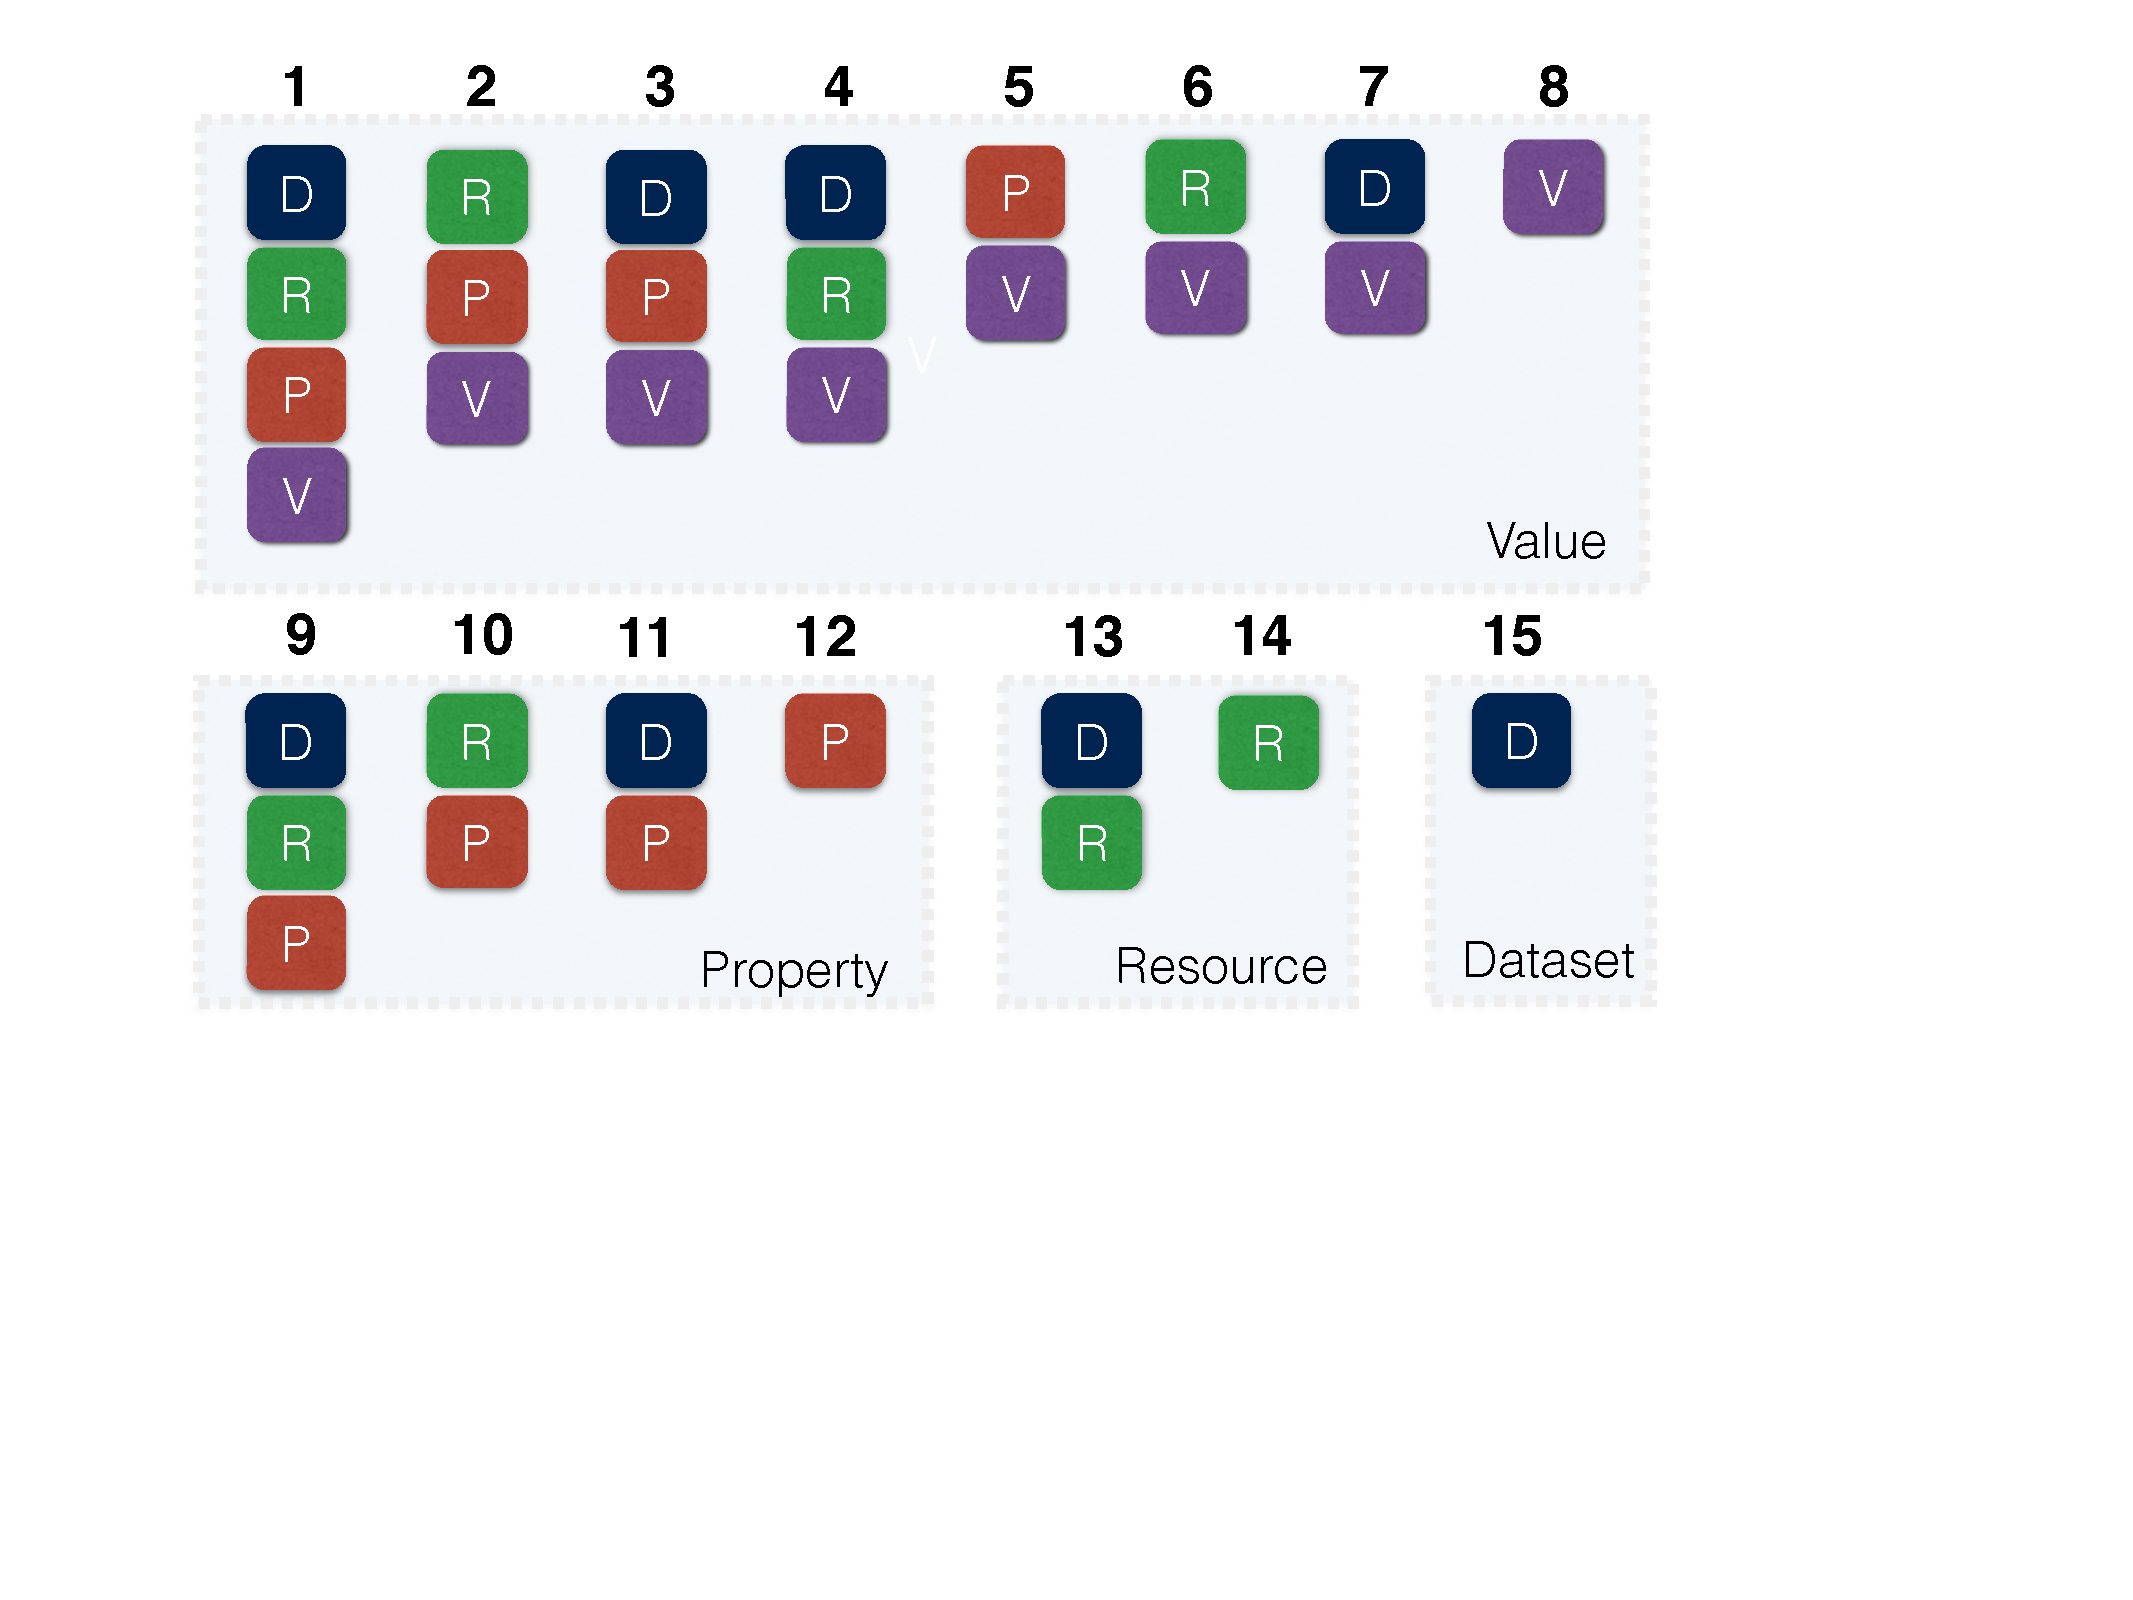
\includegraphics[width=.95\linewidth]{images/scopes.pdf}
  \caption{LD-R scopes based on the permutation of dataset, resource, property and value identifiers.}
  \label{fig:scopes}
\end{figure}

\begin{figure}[tb]
 \center
  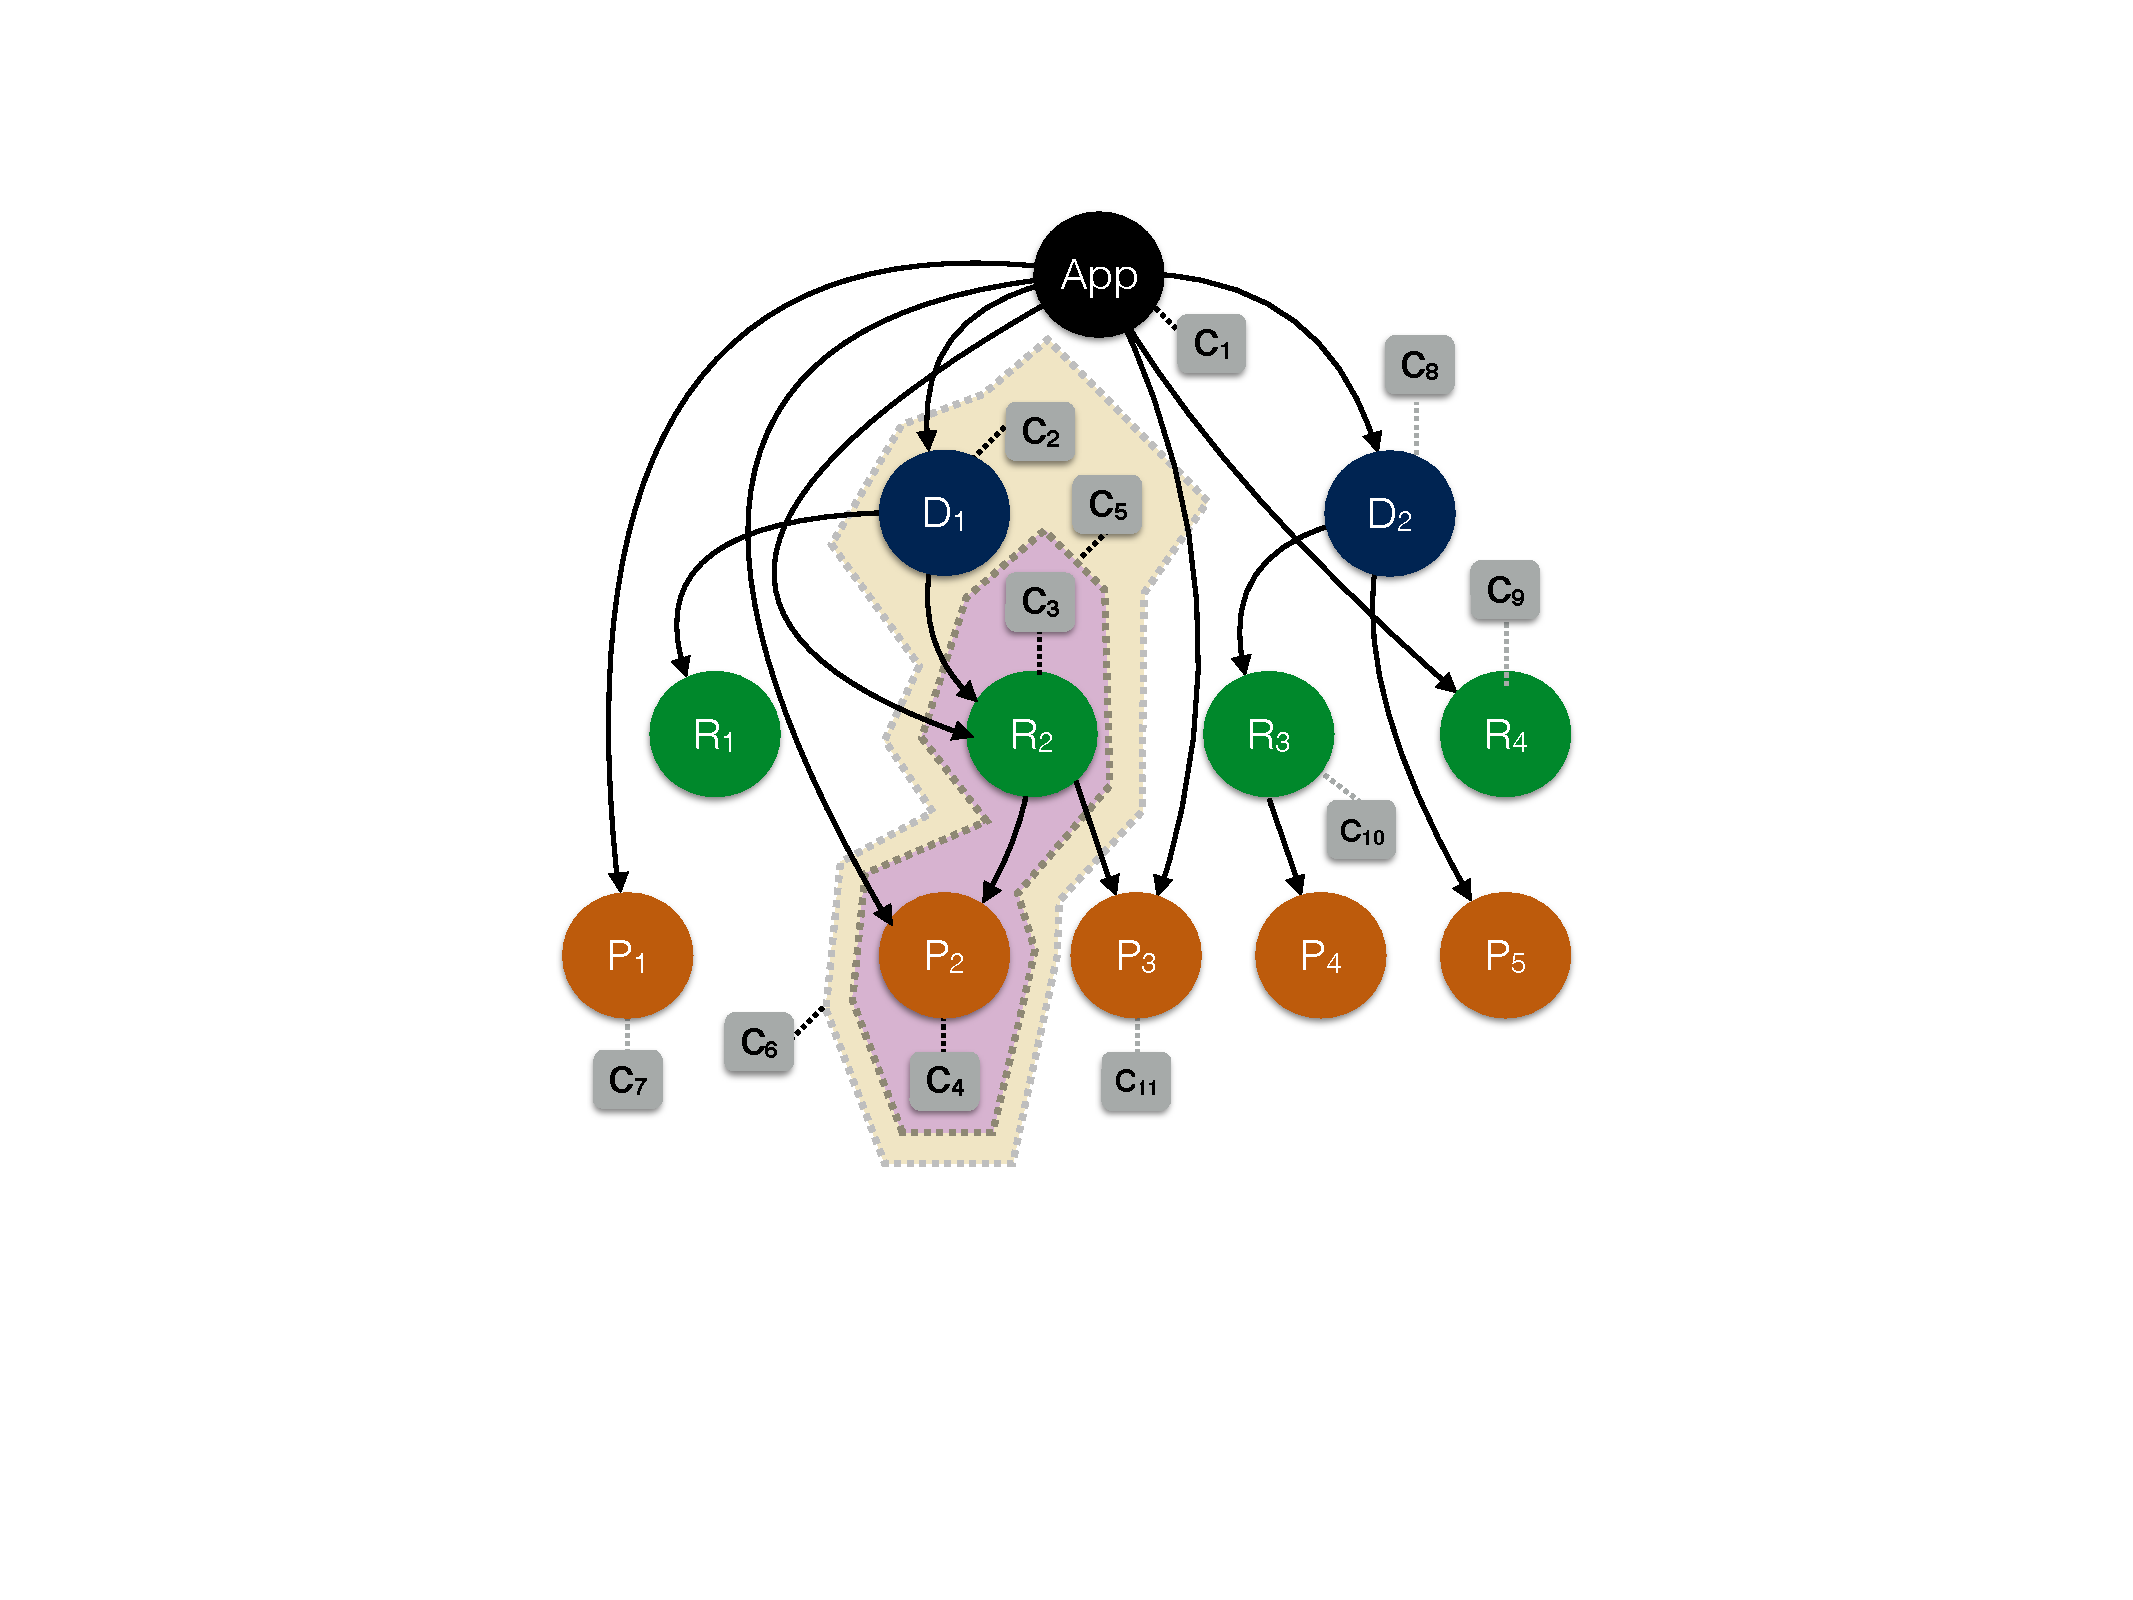
\includegraphics[width=.73\linewidth]{images/exampleConfig.pdf}
  \caption{A sample LD-R configuration hypergraph.}
  \label{fig:exampleConfig}
\end{figure}

LD-R Web components provide a versatile approach for context adaptation.
A context can be a specific domain of interest, a specific user requirement or both.
In order to enable customization and personalization, the LD-R approach exploits the concepts of \emph{Scope} and \emph{Configuration}.
A scope is defined as a hierarchical permutation of Dataset, Resource, Property and Value components (cf. \autoref{fig:scopes}).

\begin{lstlisting}[firstnumber=1, frame=tb, backgroundcolor=\color{white}, basicstyle=\small\ttfamily, label=code:adaptation, caption=Algorithm for the LD-R UI adaptation.]
InitialConfig = {initial application configuration}
Context = [array of scopes with the corresponding configuration objects]
Config = InitialConfig
for (i = 15; i < 1; i--) {
    Config.compareWith(Context[i]) {
        Config.addMissingAttributes()
        Config.overwriteExistingAttributes()
    }
}
\end{lstlisting}

Each scope conveys a certain level of specificity on a given context ranging from 1 (most specific) to 15 (least specific).
Scopes are defined by using either the URIs of named graphs, resources and properties, or by identifying the resource types and data types.
A configuration is defined as a setting which affects the way the LDA and Web components are interpreted and rendered (e.g. render a specific component for a specific RDF property or enforce a component to display Wikipedia page URIs for DBpedia resources).
UI adaptation is handled by traversing the configurations for scopes, populating the configurations and overwriting them when a more specific applicable scope is found.
As shown in \autoref{code:adaptation} below, in the worst case when the \texttt{DRPV} scopes are used and the UI is supposed to render the Value components, all 15 scopes need to be traversed for the adaptation:


\autoref{fig:exampleConfig} demonstrates an example of the LD-R configuration hypergraph containing scopes with the maximum depth of \texttt{DRP}.
The graph defines a generic configuration for the application as C$_{\text{1}}$.
There are configurations defined for the dataset scope D$_{\text{1}}$ as C$_{\text{2}}$, for the resource scope R$_{\text{2}}$ as C$_{\text{3}}$ and for the property scope P$_{\text{2}}$ as C$_{\text{4}}$.
There are also configurations for the \texttt{RP} scope R$_{\text{2}}$P$_{\text{2}}$ as C$_{\text{5}}$ and for the \texttt{DRP} scope D$_{\text{1}}$R$_{\text{2}}$P$_{\text{2}}$ as C$_{\text{6}}$.
Let's suppose we have a setting with the following values for the scopes and configurations:
\begin{compactitem}

\item
D$_{\text{1}}$= \texttt{<http://ld-r.org/users>}
\item
R$_{\text{2}}$= type \texttt{foaf:Person}
\item
P$_{\text{2}}$= \texttt{rdfs:label}
\item
C$_{\text{1}}$=\{\{viewer:`basic'\},\{attr$_{\text{1}}$:1\},\{attr$_{\text{2}}$:3\}\}
\item
C$_{\text{2}}$=\{\{attr$_{\text{1}}$:0\},\{attr$_{\text{3}}$:2\}\}
\item
C$_{\text{3}}$=\{\{attr$_{\text{3}}$:1\},\{attr$_{\text{4}}$:4\},\{attr$_{\text{5}}$:1\}\}
\item
C$_{\text{4}}$=\{\{attr$_{\text{5}}$:2\},\{attr$_{\text{6}}$:1\}\}
\item
C$_{\text{5}}$=\{\{viewer:`contact'\},\{attr$_{\text{3}}$:5\},\{attr$_{\text{7}}$:6\}\}
\item
C$_{\text{6}}$=\{\{attr$_{\text{3}}$:8\},\{attr$_{\text{7}}$:1\},\{attr$_{\text{8}}$:3\}\}
\end{compactitem}

With the above settings, when a property component for \texttt{rdfs:label} is rendered without the dataset and resource context, the configuration will be:

 \{\{viewer:`basic'\},\{attr$_{\text{1}}$:1\},\{attr$_{\text{2}}$:3\},\{attr$_{\text{5}}$:2\},\{attr$_{\text{6}}$:1\}\}

When the property component gets rendered within the resource context of type \texttt{foaf:Person}, the settings for viewer and attr$_{\text{5}}$ are overwritten and new settings for attr$_{\text{3}}$, attr$_{\text{4}}$ and attr$_{\text{7}}$ are added:

\{\{viewer:`contact'\},\{attr$_{\text{1}}$:1\},\{attr$_{\text{2}}$:3\},\{attr$_{\text{3}}$:5\},\{attr$_{\text{4}}$:4\},\newline\{attr$_{\text{5}}$:1\},\{attr$_{\text{6}}$:1\},\{attr$_{\text{7}}$:6\}\}

When the additional context of dataset as ~\texttt{<http://ld-r.org/users>} is given, attr$_{\text{3}}$ and attr$_{\text{7}}$ get overwritten and a new setting for attr$_{\text{8}}$ is added:

\{\{viewer:`contact'\},\{attr$_{\text{1}}$:0\},\{attr$_{\text{2}}$:3\},\{attr$_{\text{3}}$:8\},\{attr$_{\text{4}}$:4\},\newline\{attr$_{\text{5}}$:1\},\{attr$_{\text{6}}$:1\},\{attr$_{\text{7}}$:1\},\{attr$_{\text{8}}$:3\}\}


Scopes can also be defined on a per user basis, facilitating the versioning and reuse of user-specific configurations.
User-Specific configurations provide different views on components and thereby data, based on the different personas dealing with them.

In addition to the fine-grained component customization, LD-R Web applications provide a fine-grained access control over the data through the component scopes.
For example, an application developer can restrict access to a specific property of a specific resource in a certain dataset and on a specific interaction mode.

\subsection{Semantic Markup for Web Components}
\label{sec:markup}
The innate support of RDF in LD-R Web components enable the automatic creation of semantic markup on the UI level.
Lower semantic techniques such as \emph{RDFa}, \emph{Mircodata} and \emph{JSON-LD} can be incorporated in the core LD-R components to expose structured data to current search engines which are capable of parsing semantic markup.
For example, an LD-R component created based on the Good Relations\footnote{\url{http://www.heppnetz.de/projects/goodrelations/}} or \url{Schema.org} ontologies, can automatically expose the product data as Google Rich Snippets for products\footnote{\url{https://developers.google.com/structured-data/}} which will provide better visibility of the data on Web search results (i.e. SEO).

In addition to automatic annotation of data provided by the LD-R Web components, the approach offers semi-automatic markup of Web components by creating component metadata.
Component metadata consists of two categories of markup:
\begin{itemize}
\item Automatic markup generated by parsing component package specification -- metadata about the component and its dependencies. It includes general metadata such as name, description, version, homepage, author as well as technical metadata on component source repository and dependencies.

\item Manual markup created by component authors which exposes metadata such as component level (dataset, resource, property, value), granularity (individual, aggregate), mode (view, edit, browse) and configuration parameters specification.

\end{itemize}

Similar to content markup, Component markup can utilize commonly-known ontologies such as \url{Schema.org} in order to improve the visibility of LD-R components and enable application assemblers to better understand the intended usage and capabilities of a given component.

\begin{figure}[tb]
\center
  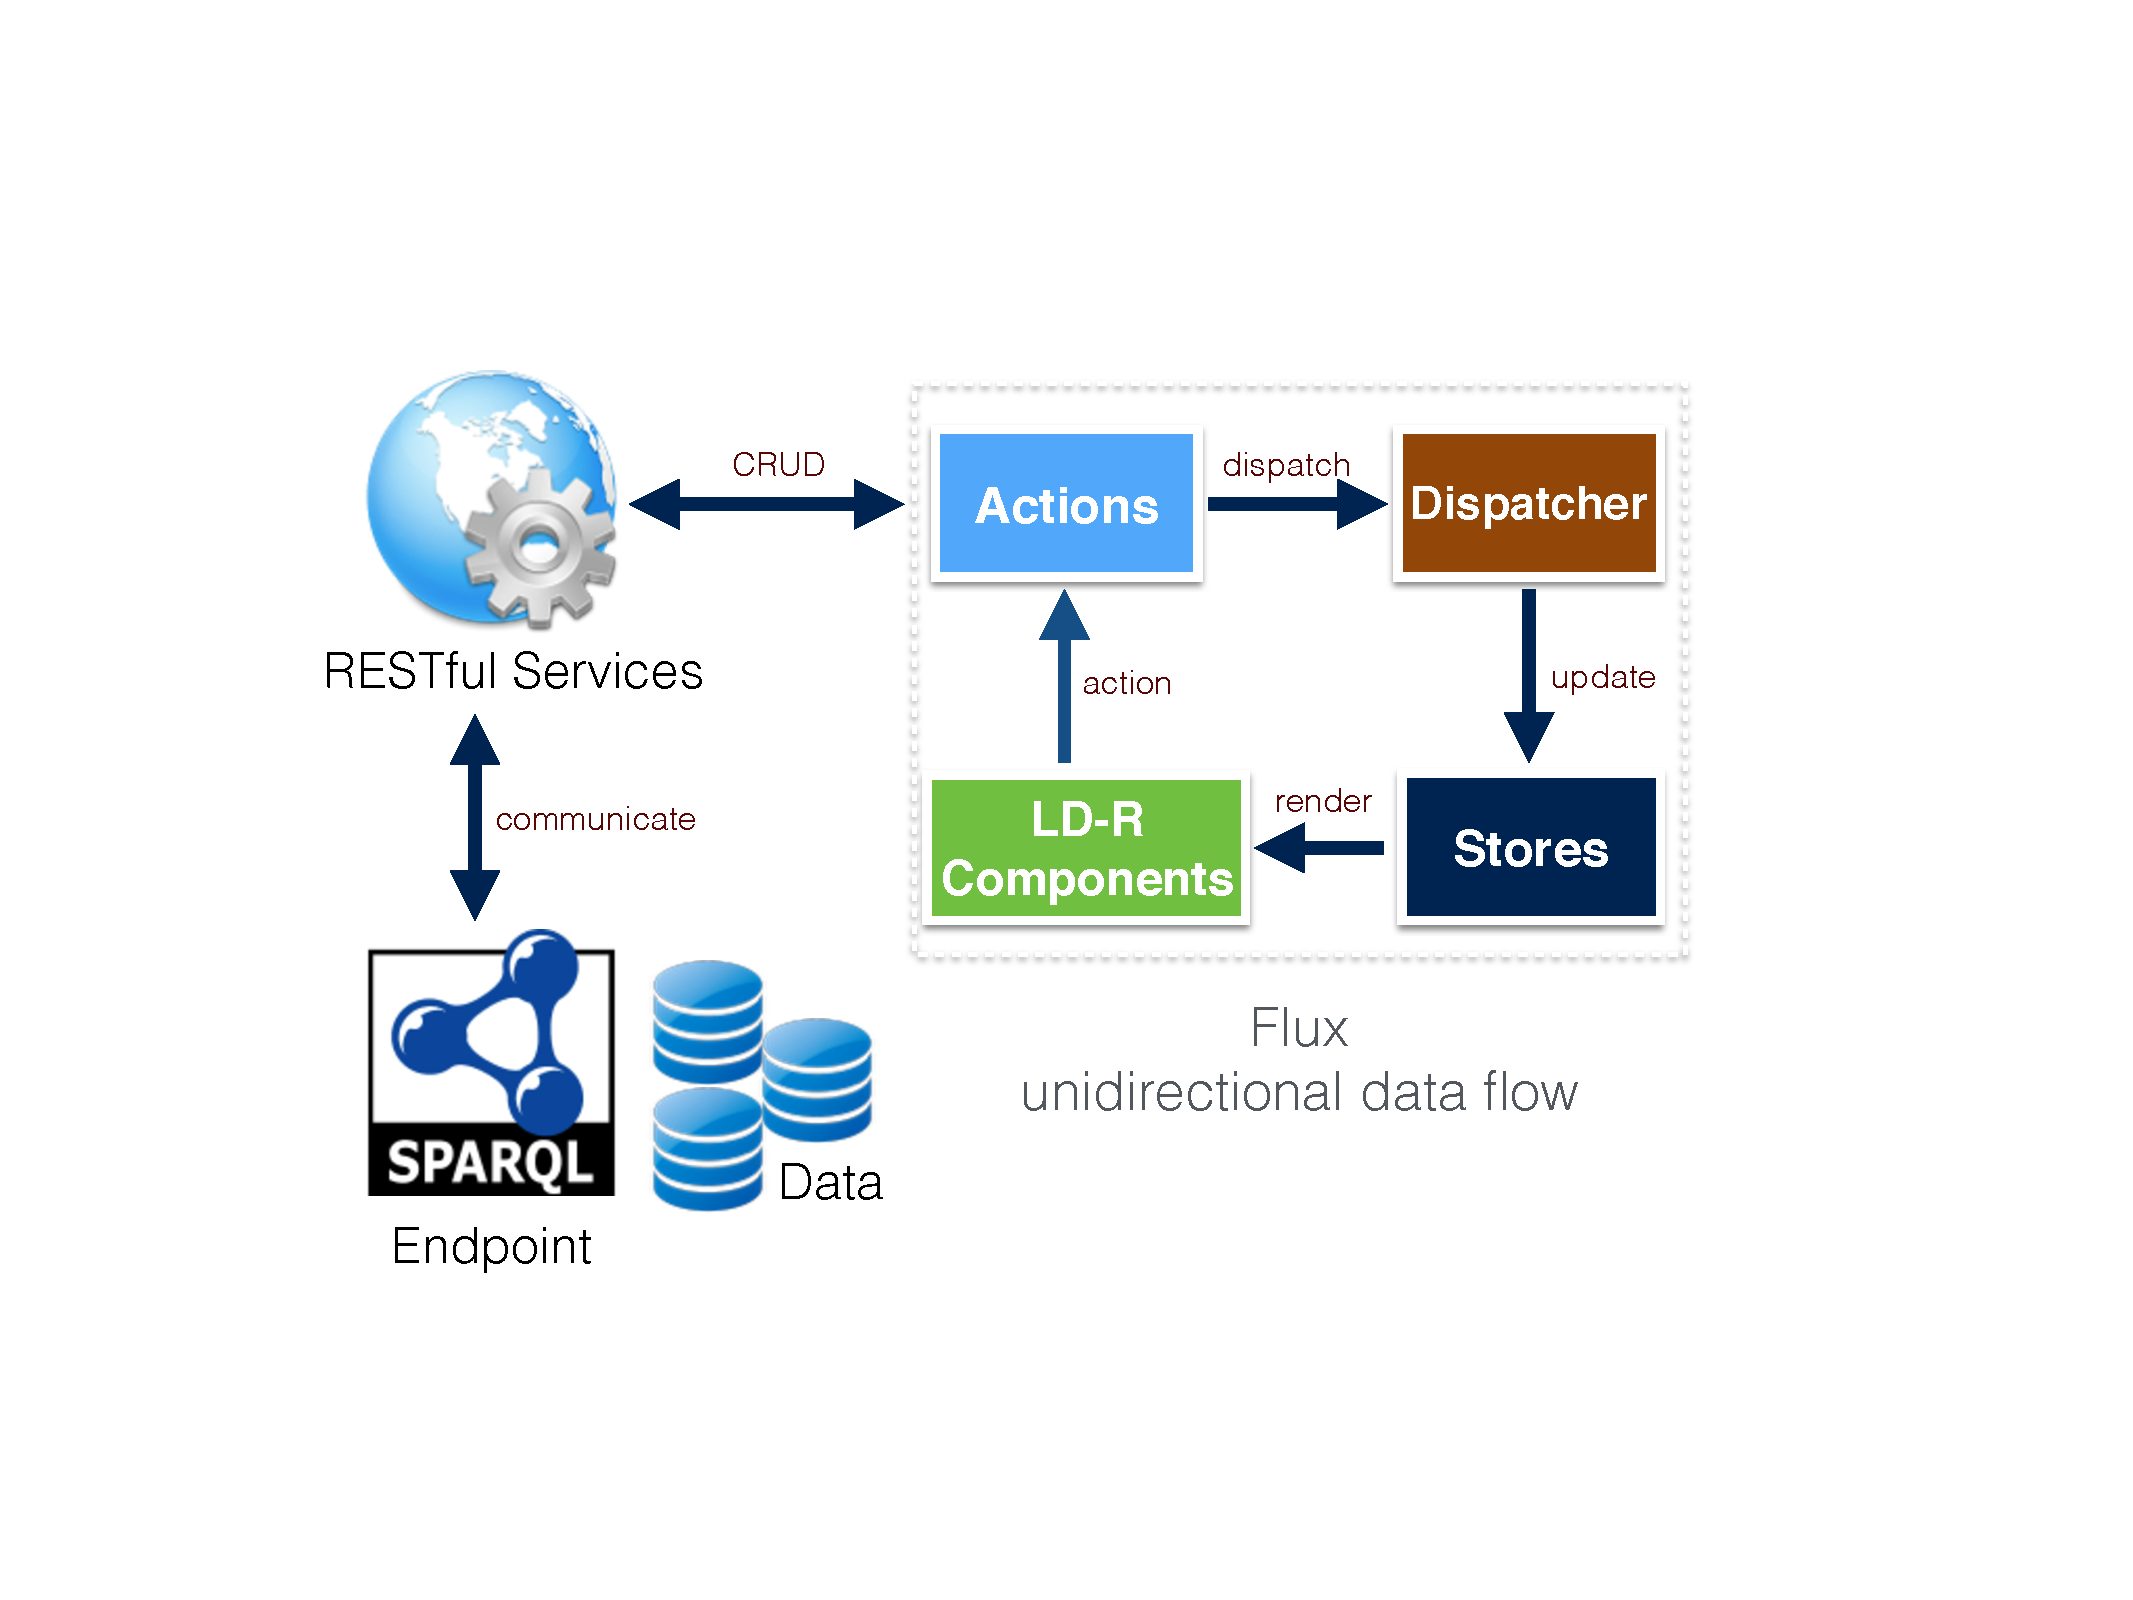
\includegraphics[width=.75\linewidth]{images/dataflow.pdf}
  \caption{Data flow in the LD-Reactor framework.}
  \label{fig:dataflow}
\end{figure}

\section{Implementation}
\label{sec:implementation}
In order to realize the idea of adaptive Linked Data-driven Web components, we implemented an open-source software framework called \emph{Linked Data Reactor (LD-Reactor)} which is available online at \url{http://ld-r.org}.
LD-Reactor utilizes Facebook's ReactJS\footnote{\url{https://facebook.github.io/react/}} components, the Flux\footnote{\url{https://facebook.github.io/flux}} architecture, Yahoo!'s Fluxible\footnote{\url{http://fluxible.io/}} framework for isomorphic Web applications (i.e. running the components code both on the server and the client) and the Semantic-UI\footnote{\url{http://semantic-ui.com/}} framework for flexible UI themes.
The main reasons we chose \emph{React} components over other  Web Components solutions (e.g. Polymer\footnote{\url{http://www.polymer-project.org/}}, AngularJS\footnote{\url{https://angularjs.org/}}, EmberJS\footnote{\url{http://emberjs.com/}}, etc.) were the maturity and maintainability of the technology, the native multi-platform support, the number of developer tools/components/applications, and the efficiency of its underlying virtual DOM approach\footnote{Elaborating on all these factors is beyond the scope of this paper.}.

As shown in \autoref{fig:dataflow}, LD-Reactor follows the Flux architecture which eschews MVC (Model-View-Controller) in favour of a unidirectional data flow.
When a user interacts with a React component, the component propagates an action through a central dispatcher, to the various stores that hold the application's data and business logic, and updates all affected components.
The component interaction with SPARQL endpoints to retrieve and update Linked Data occurs through the invocation of RESTful services in actions.

In order to allow the bootstrapping of LDA UIs, LD-Reactor provides a comprehensive framework that combines the following main elements:
\begin{itemize}

\item A set of RESTful Web services that allow basic CRUD operations on Linked Data using SPARQL queries\footnote{the framework is compliant with the SPARQL 1.1 standard. However, we have identified certain inconsistencies between OpenRDF Sesame and OpenLink Virtuoso RDF stores, which did not allow the execution of syntactically identical queries across both systems. Thereby, specific adaptors have been implemented for each of these two RDF stores.}.

\item A set of core components called \emph{Reactors} which implement core Linked Data components (see \autoref{fig:architecture}) together with their corresponding actions and stores.

\item A set of default components which allow basic viewing, editing and browsing of Linked Data.

\item A set of minimal viable configurations based on the type of data and properties from commonly-used vocabularies on the Semantic Web (e.g. foaf, dcterms and SKOS).

\item A basic access control plugin which allows restricting read/write access to data.

\end{itemize}

%\begin{figure}[htb]
%  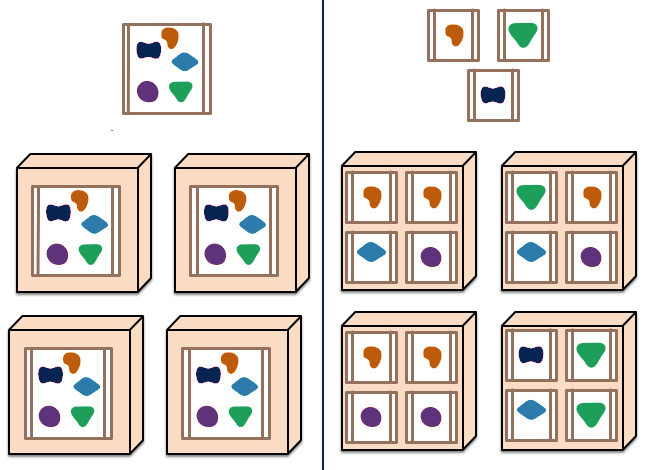
\includegraphics[width=.8\linewidth]{images/microservices.jpg}
%  \caption{Monoliths vs. Microservices~\cite{microservices}}
%  \label{fig:microservices}
%\end{figure}
%

LD-Reactor implementation is compliant with \emph{Microservices Architecture}~\cite{microservices} where the existing ReactJS components can be extended by complementary Linked Data services.
In contrast to the centralized monolithic architecture, the microservices architecture allows placing the main functionalities of the LDA into separate decoupled services and scale by distributing these services across servers, replicating as needed.
This architectural style also helps to minimize the redeploying of the entire application when changes in components were requested.

%\cite{SmartComposition2015}

\begin{figure}[htb]
  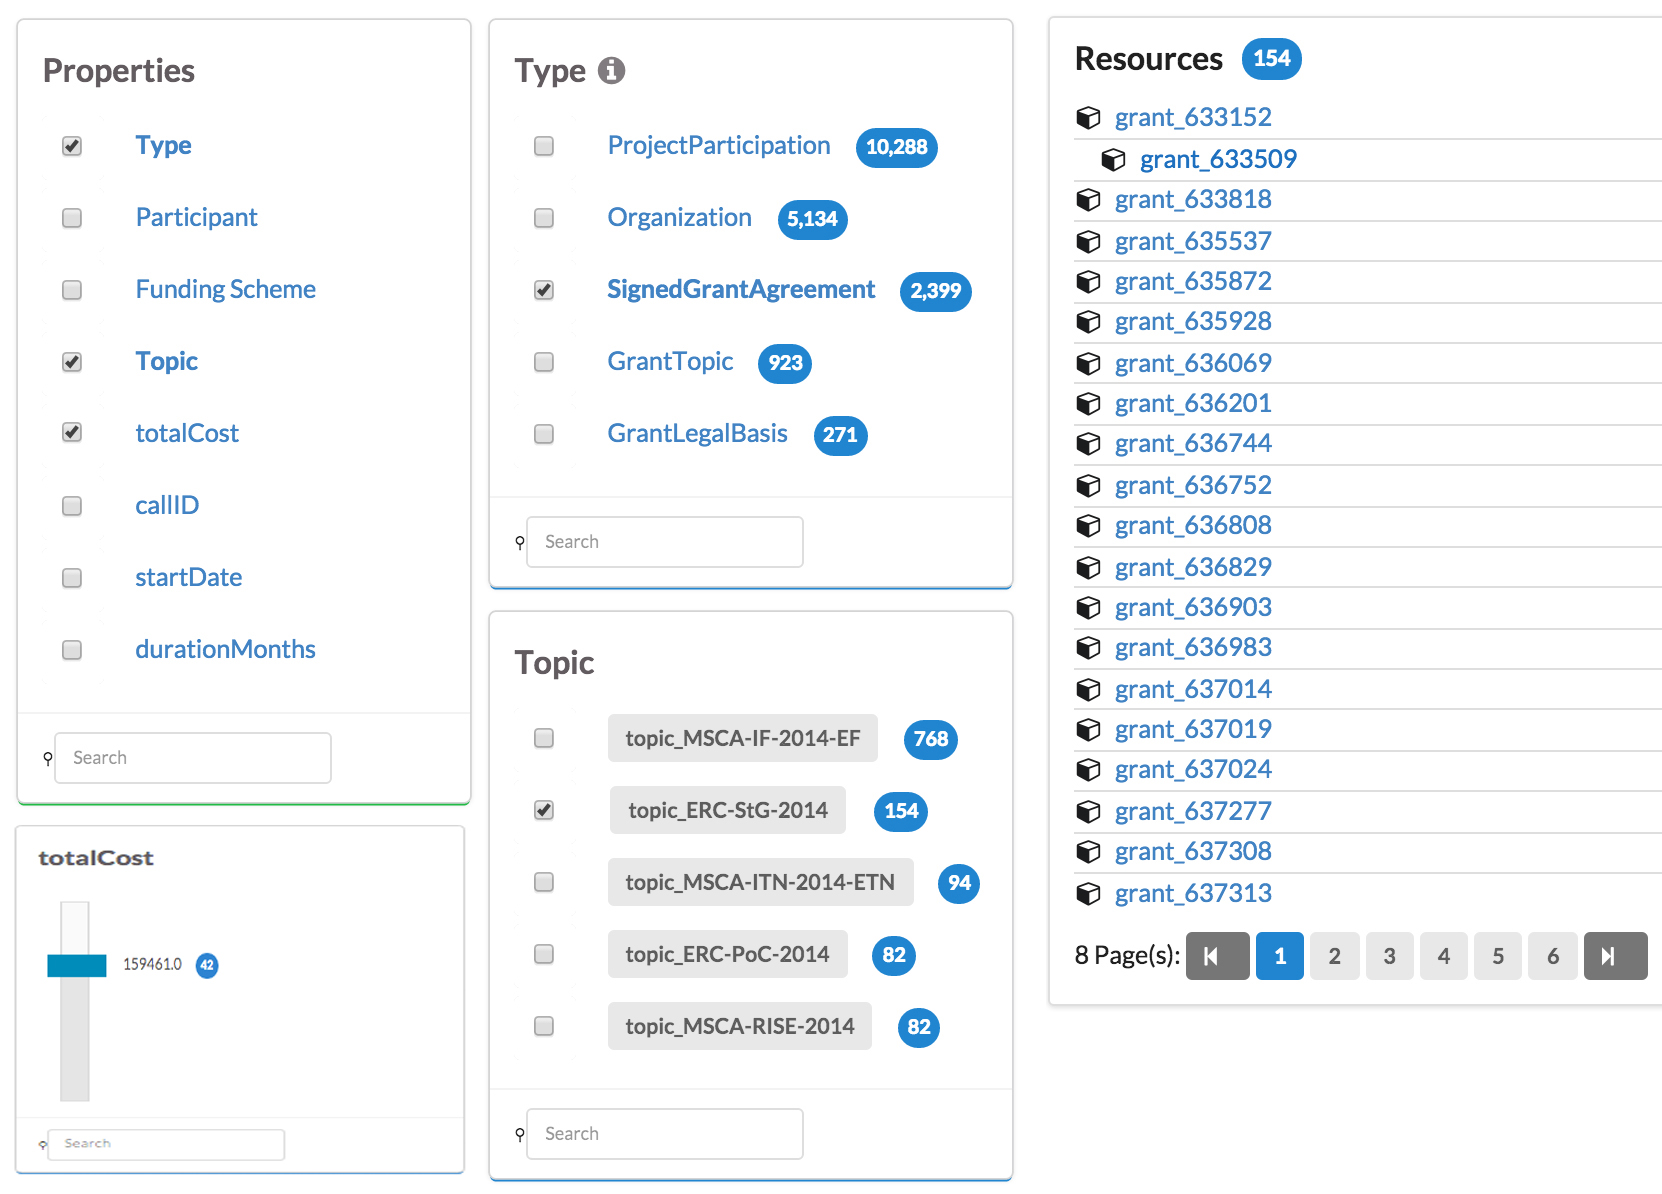
\includegraphics[width=1\linewidth]{images/facets.jpg}
  \caption{A screenshot of LD-Reactor browse mode.}
  \label{fig:ldrBrowse}
\end{figure}

There are three modes of interactions within LD-R components namely \emph{view}, \emph{browse} and \emph{edit}.
These modes work with two types of value granularity: individual and aggregate.
As shown in \autoref{fig:ldrViewEdit}, components can target individual values or interact with aggregate values when users want to show/update multiple values at once.
\autoref{fig:ldrBrowse} depicts the browse mode where individual (e.g. item lists with check boxes) and aggregate data browser (e.g. data sliders or maps) components can be employed.

Semantic markup of data (as discussed in Section \ref{sec:markup}) is supported natively within the framework by embedding Microdata annotations within the LD-R Web components.
Additionally, in order to facilitate the creation of component metadata, we developed a tool\footnote{\url{https://github.com/ali1k/ld-r-metadata-generator}} which automatically generates the general metadata about the components in JSON-LD, using \url{Schema.org}'s SoftwareApplication schema\footnote{\url{https://schema.org/SoftwareApplication}}.

\autoref{code:config} presents a sample LD-R config which is already in-use within the RISIS project\footnote{\url{http://datasets.risis.eu}}:

\begin{itemize}
 \item The UI should be able to render metadata properties in different categories (\autoref{code:config} line 3, 4).
 \item The labels for properties should be changeable in the UI especially for technical properties (e.g. RDF dump) that are unknown to researchers outside the Semantic Web domain (\autoref{code:config} line 18, 26, 40).
 \item There should be a hint for properties to help metadata editors to understand the meaning of the property (\autoref{code:config} line 20, 28, 41).
 \item Instead of showing the full URIs, the output UI should render either a shortened URI or a meaningful string linked to the original URI (\autoref{code:config} line 6).
 \item Whenever a DBpedia URI is provided, display the corresponding Wikipedia URI enabling users to retrieve human readable information (\autoref{code:config} line 33, 45).
 \item When a dropdown menu is provided, there should be the ability to accommodate user-defined values which are not listed in the menu (\autoref{code:config} line 57).

\end{itemize}

\newpage
\begin{figure}[htb]
  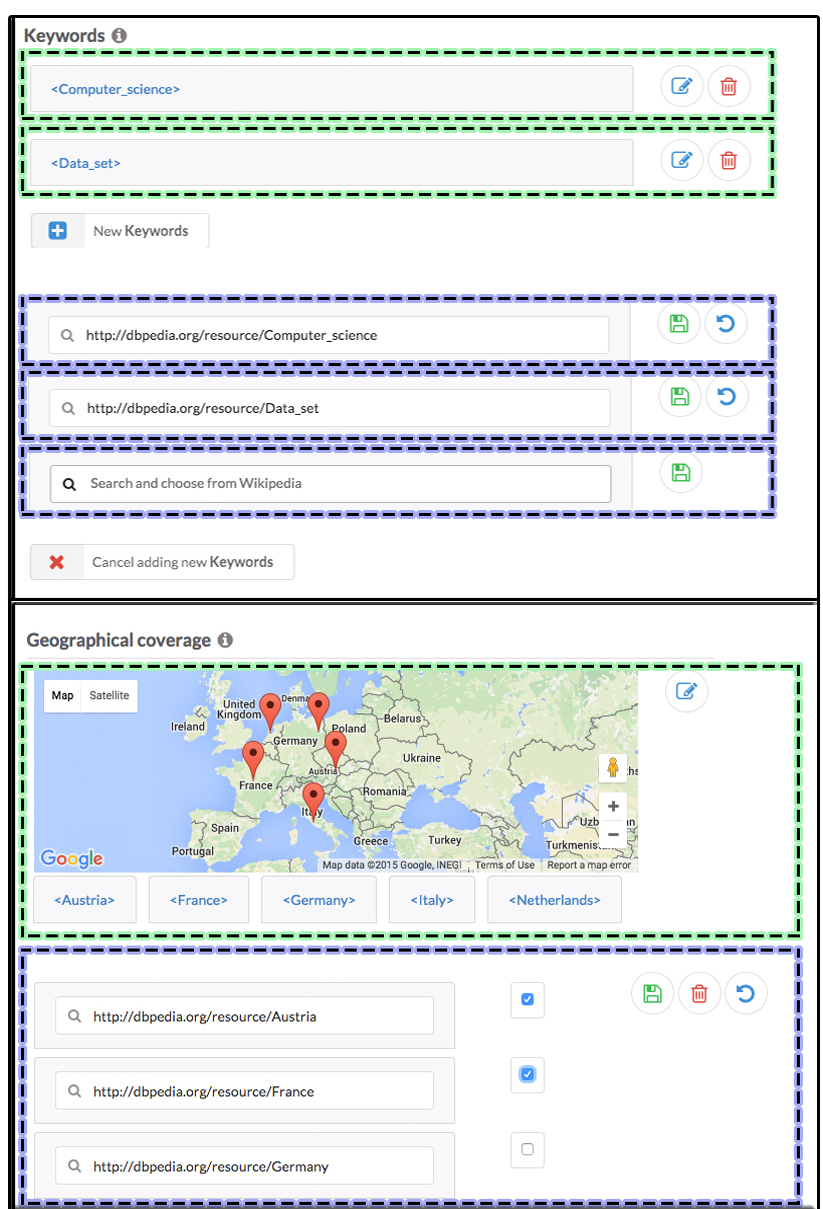
\includegraphics[width=1\linewidth]{images/viewedit.png}
  \caption{A screenshot of LD-Reactor view and edit mode for individual (top) and aggregate (bottom) values.}
  \label{fig:ldrViewEdit}
\end{figure}
\clearpage
\newpage
\begin{lstlisting}[language=json,firstnumber=1, label=code:config, caption=An excerpt of the LD-Reactor configuration file.]
resource: {
    `generic': {
        usePropertyCategories: 1,
        propertyCategories: [`overview', `legalAspects', `technicalAspects'],
        resourceReactor: [`Resource'],
        shortenURI: 1
    }
},
property: {
    `generic': {
        propertyReactor: [`IndividualProperty'],
        objectReactor: [`IndividualObject'],
        objectIViewer: [`BasicIndividualView'],
        objectIEditor: [`BasicIndividualInput']
    },
    `http://purl.org/dc/terms/language': {
        allowNewValue: 1,
        label: [`Dataset Language'],
        category: [`overview'],
        hint: [`The language of the dataset. Resources defined by the Library of Congress (http://id.loc.gov/vocabulary/iso639-1.html, http://id.loc.gov/vocabulary/iso639-2.html) SHOULD be used.'],
        objectIViewer: [`LanguageView'],
        objectIEditor: [`LanguageInput'],
        defaultValue: [`http://id.loc.gov/vocabulary/iso639-1/en']
    },
    `http://purl.org/dc/terms/spatial': {
         label: [`Geographical coverage'],
         category: [`overview'],
         hint: [`The geographical area covered by the dataset.'],
         allowNewValue: 1,
         objectReactor: [`AggregateObject'],
         objectAViewer: [`DBpediaGoogleMapView'],
         objectIViewer: [`BasicDBpediaView'],
         asWikipedia: 1,
         objectAEditor: [`BasicAggregateInput'],
         objectIEditor: [`DBpediaInput'],
         lookupClass: [`Place']
     },
    `http://purl.org/dc/terms/subject': {
        category: [`overview'],
        label: [`Keywords'],
        hint: [`Tags a dataset with a topic.'],
        allowNewValue: 1,
        objectIEditor: [`DBpediaInput'],
        objectIViewer: [`BasicDBpediaView'],
        asWikipedia: 1
    },
    `http://purl.org/dc/terms/license': {
        category: [`legalAspects'],
        label: [`License'],
        allowNewValue: 1,
        objectIViewer: [`BasicOptionView'],
        objectIEditor: [`BasicOptionInput'],
        options: [
            {label: `Open Data Commons Attribution License', value: `http://www.opendatacommons.org/licenses/by/'},
            {label: `Creative Commons Attribution-ShareAlike', value: `http://creativecommons.org/licenses/by-sa/3.0/'}
        ],
        allowUserDefinedValue: 1
    }
}
\end{lstlisting}

\section{Related Work}
We have brought an elaborate analysis of the related work in \cite{khaliliLDR2016}. In this section, we only summarize the main related work.

\paragraph{UI Frameworks.}
WYSIWYM (What You See Is What You Mean)~\cite{WYSIWYM2014} is a generic semantics-based UI model to allow integrated visualization, exploration and authoring of structured and unstructured data.
Our proposed approach utilizes the WYSIWYM model for binding RDF-based data to viewer, editor and browser UIs.
Uduvudu~\cite{Uduvudu2015} is another approach to making an adaptive RDF-based UI engine to render Linked Data.
Instead of adopting Web components, Uduvudu employs a set of flexible UI templates that can be combined to create complex UIs.
Even though the static templates do not provide enough interactions for editing and browsing data (in contrast to Web components), we believe that algorithms for automatic selection of templates employed in Uduvudu can be reused in the LD-Reactor framework for automatic generation of configurations.
Another similar approach is SemwidgJS~\cite{StegemannZ14} which brings a semantic Widget library for the rapid development of LDA UIs.
SemwidgJS offers a simplified query language to allow the navigation of graph-based data by ordinary Web developers.
The main difference between LD-R and SemwidgJS is that LD-Reactor suggests a more interactive model which is not only for displaying Linked Data but also for providing user adaptations based on the meaning of data.
LD-Viewer~\cite{Lukovnikov2014} is another related Linked Data presentation framework particularly tailored for the presentation of DBpedia resources.
In contrast to LD-Reactor, LD-Viewer  builds on top of the traditional MVC architecture and its extensions rely heavily on the knowledge of RDF which is a burden for developers unfamiliar with Semantic Web technologies.

\paragraph{Tools and Applications.}
In addition to the LDA UI frameworks, there are several ad-hoc tools for Linked Data visualization and exploration such as Balloon Synopsis~\cite{BalloonSchlegelWSGK14} and Sgvizler~\cite{Sgvizler} which can  be utilized as Web components within the LD-Reactor framework.
\cite{Abascal2015} provides an extensive list of these tools aiming to make Linked Data accessible for common end-users who are not familiar with Semantic Web.

Overall, what distinguishes Linked-Data-Reactor from the existing frameworks and tools is its modern isomorphic component-based architecture that addresses reactive and reusable UIs as its first class citizen.


\section{Conclusion}
We argue that bridging the gap between Semantic Web Technologies and Web Components worlds brings mutual benefits for both sides.
On one hand, Semantic Web technologies provide support for richer component discovery, interoperability, integration, and adaptation on the Web.
On the other, Web Components bring the advantages of UI standardization, reusability, replaceability and encapsulation to current Semantic Web applications.

This paper presented Linked Data Reactor as a component-based LDA development framework which aims to bring a better communication between UX designers and Semantic Web developers in order to reuse best UI practices within Linked Data applications.

%\clearpage

\bibliographystyle{abbrv}
\scriptsize
\bibliography{refs}

\end{document}
